\chapter{Interactions}

In many analyses we may consider that the effect of $x$ on $y$ is moderated by a third variable, $z$. That is to say, the slope of $x$ may be different depending on the level or value of $z$. These ideas can be tested in a regression framework through interactions. An interaction between two variables, $a$ and $b$ is simply the product of the variables, which can be noted as $a\times b$.

\section{Interactions between categorical predictors}

First, consider a model in which $y$ is a function of two categorical predictors, $x$, and $z$. Each predictor takes on two values (0 and 1). Suppose some variable $y$ was a function of both of these variables, and that these variables interacted in some way to produce effects greater than the combination of their marginal effects. That is to say, $x$ has an effect when $x=1$, $z$ has an effect when $z=1$, but when $x$ and $z$ both are 1, there is an additional effect.

Consider Table~\ref{tab:caty}, in which I report the mean of $y$ for different values of $x$ and $z$, as well as the marginals. We can fit a model to estimate the difference between $x=0$ and $x=1$ regardless of the level of $z$:
\[
y_i = \beta_0+\beta_1x_i+e_i
\]
Where $\beta_0$ is the average of $y$ when $x=0$ and $\beta_1$ is the difference between $\hat{y}|x=1$ and $\hat{y}|x=0$, or $\beta_1 = \left(\hat{y}|x=1\right) - \left(\hat{y}|x=0\right)$. Model 1 in Table~\ref{tab:catyreg} gives this effect (with some rounding error in the third decimal).

\begin{table}[htbp]\centering
\caption{Means of $y$ across two categorical predictors \label{tab:caty}
\textbf{} }\begin{tabular} {@{} rrrr @{}} \\
 & $z = 0$ & $z = 1$ & All $z$ \\
\hline
$x = 0$ &  0.449 & -1.158 & -0.355 \\
$x = 1$ & -0.977 & 0.290 & -0.343 \\
\hline
All $x$ & -0.264 & -0.434 & -0.349 \\
\hline
\multicolumn{4}{@{}l}{$N=400$, balanced data\footnotesize{\emph{} }}
\end{tabular}
\end{table}

Likewise, we can fit a model to estimate the difference between $z=0$ and $z=1$ regardless of the level of $x$:
\[
y_i = \beta_0+\beta_1z_i+e_i
\]
Where $\beta_0$ is the average of $y$ when $z=0$ and $\beta_1$ is the difference between $\hat{y}|z=1$ and $\hat{y}|z=0$, or $\beta_1 = \left(\hat{y}|z=1\right) - \left(\hat{y}|z=0\right)$. Model 2 in Table~\ref{tab:catyreg} gives this effect (with some rounding error in the third decimal).

Note that in both cases, the intercept is the mean of $y$ when the predictors are zero. In this case, $x$ and $z$ are independent, and so the effects in Model 3
\[
y_i=\beta_0+\beta_1x_i+\beta_2z_i
\]
do not change. Unfortuneatly, the intercept, $\beta_0$, does not equal any of the cells.

However, we can compare the mean of $y$ when $x=0$ and $z=0$, with the mean of $y$ when $x=1$ and $z=0$, with the mean of $y$ when $x=0$ and $z=1$, and the mean of $y$ when $x=1$ and $z=1$, using an interaction. Thus, we fit Model 4 in Table~\ref{tab:catyreg}:
\[
y_i=\beta_0+\beta_1x_i+\beta_2z_i+\beta_3\left(x_i\times z_i\right)
\]

In Models 1, 2, and 3, none of the effects were significant. In Model 4, we see that we have an effect for $x$, and effect for $z$, and an interaction effect for $x_i\times z_i$. With this model, we are able to reproduce each cell in the table.\footnote{note: there is some rounding error}
\[
\left(\hat{y}|x=0,z=0\right)=\beta_0=0.449
\]
\[
\left(\hat{y}|x=1,z=0\right)=\beta_0+\beta_1=0.449+-1.429=0.977
\]
\[
\left(\hat{y}|x=0,z=1\right)=\beta_0+\beta_2=0.449+-1.606=-1.158
\]
\[
\left(\hat{y}|x=1,z=1\right)=\beta_0+\beta_1+\beta_2+\beta_3=0.449+-1.429+-1.606+2.873=0.290
\]
Note that interactions can be interpreted in the number of ways that we have variables interacting. For example, $\beta_3$ can be interpreted as the way the effect of $x$ changes when $z$ is equal to 1. That is to say, we can think of $\beta_3$ as
\[
\left(\frac{\Delta y}{\Delta x}\vert z=0\right)=\beta_1
\]
and
\[
\left(\frac{\Delta y}{\Delta x}\vert z=1\right)=\beta_1+\beta_3
\]
Similarly, $\beta_3$ can be interpreted as the way the effect of $z$ changes when $x$ is equal to 1.
\[
\left(\frac{\Delta y}{\Delta z}\vert x=0\right)=\beta_2
\]
and
\[
\left(\frac{\Delta y}{\Delta z}\vert x=1\right)=\beta_2+\beta_3
\]
In both cases, it is $\beta_3$ that is making the difference.
\begin{table}[htbp]\centering
\caption{Models predicting $y$ as a function of categorical predictors in for data in Table~\ref{tab:caty}
\label{tab:catyreg}}
\begin{tabular}{lcccc}
\hline
Coefficients&   Model 1  &   Model 2  &     Model 3  &    Model 4  \\
\hline
$x$     &    0.011  &        &    0.011  &   -1.425***\\
      &   (0.129)  &        &   (0.129)  &   (0.151)  \\
$z$     &        &   -0.170  &   -0.170  &   -1.606***\\
      &        &   (0.129)  &   (0.129)  &   (0.151)  \\
$x\times z$   &        &        &        &    2.873***\\
      &        &        &        &   (0.214)  \\
Intercept    &   -0.355***&   -0.264** &   -0.270* &    0.449***\\
      &   (0.091)  &   (0.091)  &   (0.111)  &   (0.107)  \\
\hline
\multicolumn{5}{l}{$SE$s in parentheses, $* p < 0.05, ** p < 0.01, ***p<0.001$} \\
\hline
\end{tabular}
\end{table}
\subsection{Example of categorical interactions on math scores}
  I used the Early Childhood Longitudinal Study, Kindergarten class of 1998-1999 to estimate the effects of gender and race on math scores for kindergartners. The math scores were standardized to allow the slope coefficients to represent changes in standard deviations. Model 1 in Table~\ref{tab:eclsinter} presents the following model where math is a function of gender:
\[
math_i=\beta_0+\beta_1female_i+e_i
\]
Model 2 presents the following model where math is a function of race:
\[
math_i=\beta_0+\beta_1black_i+e_i
\]
Model 3 presents the following model where math is a function of gender and race:
\[
math_i=\beta_0+\beta_1female_i+\beta_2black_i+e_i
\]
and Model 4 presents the following model where math is a function of gender, race, and the interaction of gender and race:
\[
math_i=\beta_0+\beta_1female_i+\beta_2black_i+\beta_3\left(female_i\times black_i\right)+e_i.
\]
We first interpret Model 1. Recalling that the intercept, $\beta_0$, is always the value of $y$ when all predictors are zero, we interpret that standardized math scores are equal to about 0.014 for {\it male} students, and that {\it female} students' math scores are 0.027 standard deviations lower, on average, than {\it male} students. However, this finding is not statistically signifiant, with a $t$-value of
\[
t=\frac{\beta_1}{SE\left(\beta_1\right)}=\frac{-0.027}{0.019}=-1.42
\]
which has a probability, or $p$-value, of 0.078, which is greater than the threshold of $\alpha = 0.05$. Thus, the effect is not significant.
\begin{table}[htbp]\centering
\caption{Model predicting kindergartner math scores as a function of gender and race
\label{tab:eclsinter}}
\begin{tabular}{lcccc}
\hline
Coefficients&Model 1&Model 2&Model 3&Model 4 \\
\hline
female   &   -0.027  &        &   -0.021  &   -0.035  \\
      &   (0.019)  &        &   (0.019)  &   (0.020)  \\
black    &        &   -0.501***&   -0.500***&   -0.570***\\
      &        &   (0.032)  &   (0.032)  &   (0.046)  \\
female$\times$black &        &        &        &    0.134* \\
      &        &        &        &   (0.064)  \\
Intercept    &    0.014  &    0.050***&    0.060***&    0.067***\\
      &   (0.014)  &   (0.010)  &   (0.014)  &   (0.014)  \\
\hline
\multicolumn{5}{l}{Model Statistics} \\
\hline
$F$ 							 &    2.018  &   244.643  &   122.955  &   83.456  \\
$R^2$ 						 &    0.000  &    0.022  &    0.022  &    0.023  \\
$df$ Regression 			 &    1.000  &    1.000  &    2.000  &    3.000  \\
$df$ Error 					 &  10694.000  &  10694.000  &  10693.000  &  10692.000  \\
\hline
\multicolumn{5}{l}{Math score standardized, N= 10696} \\
\multicolumn{5}{l}{$SE$s in parentheses, $***p<0.001$}{\footnotesize{\emph{Source: ECLS-K}}} \\
\hline
\end{tabular}
\end{table}
Turning to Model 2, we interpret that standardized math scores are equal to about 0.050 for {\it non-Black} students, and that {\it Black} students' math scores are 0.501 standard deviations lower, on average. This finding is statistically signifiant with $p$-value of less than 0.001, and is marked as such in the table with three stars ($***$).

Model 3 presents both variables, $female$ and $black$ as predictors, and we find again that the effect of being female is not significant, but the effect of being Black is, again estimating a gap of about half a standard deviation.

Model 4 is more interesting, introducing the interaction between race and gender. We now have four groups of students and their means: Non-Black males, Non-Black females, Black males, and Black females.  The estimated mean of Non-Black males is calculated as
\[
\hat{y}=\beta_0+\beta_1\left(female\right)+\beta_2\left(black\right)+\beta_3\left(female \times black\right)
\]
\[
\hat{y}=\beta_0+\beta_1\left(0\right)+\beta_2\left(0\right)+\beta_3\left(0 \times 0\right)
\]
\[
\hat{y}=\beta_0
\]
\[
\hat{y}=0.067
\]
The intercept is now the mean of non-Black males, with an average score of 0.067. The mean of Non-Black females is
\[
\hat{y}=\beta_0+\beta_1\left(female\right)+\beta_2\left(black\right)+\beta_3\left(female \times black\right)
\]
\[
\hat{y}=\beta_0+\beta_1\left(1\right)+\beta_2\left(0\right)+\beta_3\left(1 \times 0\right)
\]
\[
\hat{y}=\beta_0+\beta_1
\]
\[
\hat{y}=0.067+-0.035=0.032
\]
However, since $\beta_1$ is not significant, the difference between non-Black males and females is not statistically significant. Turning to Black males, we find that the predicted mean is
\[
\hat{y}=\beta_0+\beta_1\left(female\right)+\beta_2\left(black\right)+\beta_3\left(female \times black\right)
\]
\[
\hat{y}=\beta_0+\beta_1\left(0\right)+\beta_2\left(1\right)+\beta_3\left(0 \times 1\right)
\]
\[
\hat{y}=\beta_0+\beta_2
\]
\[
\hat{y}=0.067+-0.570=-0.503
\]
Finally, the mean for Black females is
\[
\hat{y}=\beta_0+\beta_1\left(female\right)+\beta_2\left(black\right)+\beta_3\left(female \times black\right)
\]
\[
\hat{y}=\beta_0+\beta_1\left(1\right)+\beta_2\left(1\right)+\beta_3\left(1 \times 1\right)
\]
\[
\hat{y}=\beta_0+\beta_1+\beta_2+\beta_3
\]
\[
\hat{y}=0.067+-0.035+-0.57+0.134=-0.404
\]
Thus, because of the interaction between $female$ and $black$, we find that among Black students, the gap in math scores is less for females than it is for males. That is to say, gender moderates the effect of race on math scores.

\section{Interactions between a categorical and a continuous predictor}

More often than interactions between categorical predictors is the wish to see if the effect of a continuous predictor is moderated by membership in a particular group. For example, suppose we had three groups of observations, Group 1, Group 2, and Group 3, and that we had some outcome variable $y$ and predictor of interest, $x$. Such a data is presented in Table~\ref{tab:groupxy}.

\begin{table}[htbp]\centering
\caption{Small dataset of random variables from three groups \label{tab:groupxy}
\textbf{} }\begin{tabular} {@{} rrrrrrrr @{}} \\
\multicolumn{2}{@{}c}{Group 1} & & \multicolumn{2}{@{}c}{Group 2} & & \multicolumn{2}{@{}c}{Group 3} \\
$y$ & $x$ & \textbf{} & $y$ & $x$ & \textbf{} & $y$ & $x$ \\
\hline
30.97 & 8.14 & & 70.69 & 8.98 & & 16.81 & 18.98 \\
18.97 & 9.02 & & 74.53 & 8.91 & & 21.07 & 18.91 \\
28.00 & 8.16 & & 79.28 & 11.20 & & 12.09 & 21.20 \\
32.02 & 10.58 & & 66.17 & 8.22 & & 16.84 & 18.22 \\
42.92 & 10.82 & & 69.19 & 10.47 & & 6.37 & 20.47 \\
30.26 & 7.78 & & 61.24 & 6.11 & & 24.59 & 16.11 \\
37.75 & 10.79 & & 82.44 & 11.37 & & 14.20 & 21.37 \\
28.87 & 8.34 & & 72.89 & 10.09 & & 12.37 & 20.09 \\
33.99 & 10.70 & & 79.51 & 11.89 & & 8.18 & 21.89 \\
41.90 & 13.50 & & 80.01 & 12.35 & & 5.93 & 22.35 \\
\hline
\multicolumn{2}{@{}l}{\footnotesize{\emph{} }}
\end{tabular}
\end{table}

We then plot each group onto the same scatterplot in Figure~\ref{fig:interscatter}, with Group 1 as circles, Group 2 as triangles, and Group 3 as squares. Overall, it appears that there is a negative relationship between $x$ and $y$, but closer inspection reveals that Groups 1 and 2 appear to have a positive relationship between $x$ and $y$. How can we decompose this information? First, we create dichotomous indicators $d_2$ and $d_3$, where
\[
d_2 = \left\{ \begin{array}{ll}
     1 & \mbox{if $Group = 2$};\\
     0 & \mbox{otherwise}.\end{array} \right.
\]
and
\[
d_3 = \left\{ \begin{array}{ll}
     1 & \mbox{if $Group = 3$};\\
     0 & \mbox{otherwise}.\end{array} \right.
\]
using Group 1 as the reference group.
\begin{figure}
   \centering
   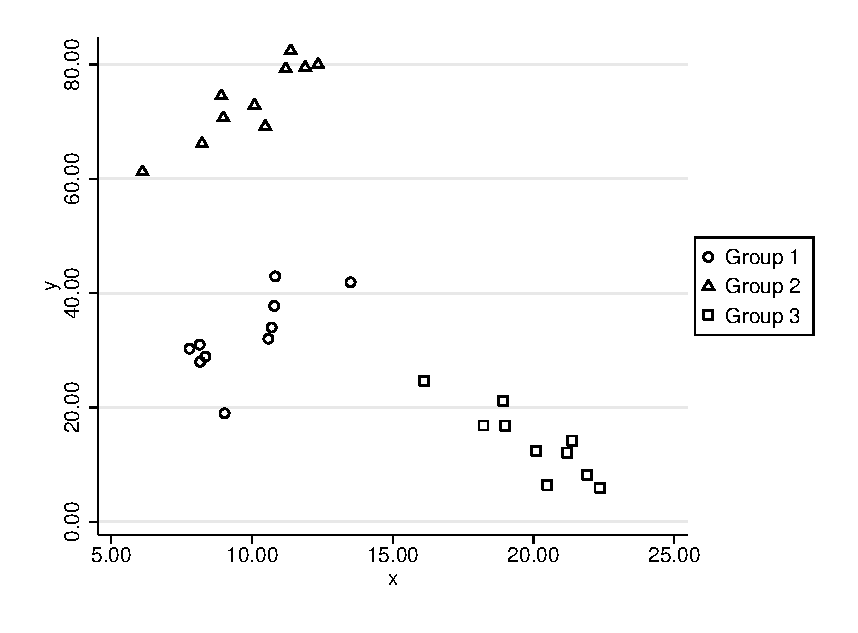
\includegraphics[angle=0,
           width=.75\textwidth]{interscatter.eps}
   \caption{Scatter plot of data in Table~\ref{tab:groupxy}}
  \label{fig:interscatter}
\end{figure}
We then explore the data with a series of models in Table~\ref{tab:interreg}. The first model is simply a bivariate model of $y$ on $x$,
\[
y_i=\beta_0+\beta_1x_i+e_i
\]
The second model adjusts the intercept of the bivariate relationship by entering the dichotomous indicators $d_2$ and $d_3$,
\[
y_i=\beta_0+\beta_1x_i+\beta_2d_{2i}+\beta_3d_{3i}+e_i
\]
and finally, the third model enters interactions of $x$ with $d_2$ and $d_3$,
\[
y_i=\beta_0+\beta_1x_i+\beta_2d_{2i}+\beta_3d_{3i}+\beta_4\left(d_{2i}\times x_i\right)+\beta_5\left(d_{3i} \times x_i\right)+e_i
\]

\begin{table}[htbp]\centering
\caption{Models from data in Table~\ref{tab:groupxy}
\label{tab:interreg}}
\begin{tabular}{lccc}
\hline
Coefficients&Model 1&Model 2&Model 3 \\
\hline
$x$     &   -3.238***&    0.998  &    2.784***\\
      &   (0.737)  &   (0.671)  &   (0.742)  \\
$d_2$  &        &   40.855***&   36.338** \\
      &        &   (2.938)  &  (10.220)  \\
$d_3$  &        &   -28.875***&   64.276***\\
      &        &   (7.434)  &  (15.833)  \\
$d_2 \times x$  &        &        &    0.422  \\
      &        &        &   (1.020)  \\
$d_3 \times x$  &        &        &   -5.578***\\
      &        &        &   (1.020)  \\
Intercept  &   82.854***&   22.799** &    5.328  \\
      &  (10.447)  &   (6.887)  &   (7.373)  \\
\hline
\multicolumn{4}{l}{$SE$s in parentheses, $**p<0.01$, $***p<0.001$} \\
\hline
\end{tabular}
\end{table}
Model 1 in Table~\ref{tab:interreg} reports a negative relationship between $x$ and $y$. This is confirmed in the first panel of Figure~\ref{fig:interfit}, where we see the fit line sloping downward. While this describes the bivariate relationship, our inspection of the data revealed a positive relationship for Groups 1 and 2.

We then fit Model 2, and work to understand exactly what the effects of $d_2$ and $d_3$ are doing. Starting with Group 1. We can find the group specific regression model for Group 1 by plugging values
\[
\hat{y}=\beta_0+\beta_1x+\beta_2d_{2}+\beta_3d_{3}
\]
\[
\hat{y}=\beta_0+\beta_1x+\beta_20+\beta_30
\]
\[
\hat{y}=\beta_0+\beta_1x
\]
and we find that the terms for $d_2$ and $d_3$ drop off.

We then move to Group 2. We can again eliminate some coefficients by simply plugging in numbers to the regression model
\[
\hat{y}=\beta_0+\beta_1x+\beta_2d_{2}+\beta_3d_{3}
\]
\[
\hat{y}=\beta_0+\beta_1x+\beta_21+\beta_30
\]
\[
\hat{y}=\beta_0+\beta_1x+\beta_2
\]
Since $\beta_0$ and $\beta_2$ are constants, we can gather terms to create an adjusted intercept
\[
\hat{y}=\left(\beta_0+\beta_2\right)+\beta_1x
\]
Therefore, the intercept for Group 2 in Model 2 in Table~\ref{tab:interreg} is $\beta_0+\beta_2$. We can do the same for Group 3:
\[
\hat{y}=\beta_0+\beta_1x+\beta_2d_{2}+\beta_3d_{3}
\]
\[
\hat{y}=\beta_0+\beta_1x+\beta_20+\beta_31
\]
\[
\hat{y}=\beta_0+\beta_1x+\beta_3
\]
\[
\hat{y}=\left(\beta_0+\beta_3\right)+\beta_1x
\]
and we find that the intercept for Group 3 in Model 2 in Table~\ref{tab:interreg} is $\beta_0+\beta_3$. Yet, in each case, the slope is $\beta_1$. That means that each group should have its own intercept, but the same slope. That is, the model for Group 1 is
\[
\hat{y}=\beta_0+\beta_1x
\]
\[
\hat{y}=22.799+0.998x
\]
and Group 2 is
\[
\hat{y}=\left(\beta_0+\beta_2\right)+\beta_1x
\]
\[
\hat{y}=\left(22.799+40.855\right)+0.998x
\]
\[
\hat{y}=63.564+0.998x
\]
and Group 3 is
\[
\hat{y}=\left(\beta_0+\beta_3\right)+\beta_1x
\]
\[
\hat{y}=\left(22.799+-28.875\right)+0.998x
\]
\[
\hat{y}=-6.076+0.998x
\]
This draws three parallel lines, and we can see that in the second panel of Figure~\ref{fig:interfit}. The problem with Model 2, however, is that the slope is not significant. We then move to Model 3 where we interact $x$ with $d_2$ and $d_3$.

Understanding models with such interactions is tractable when we perform the same "plug and chug" procedure as in the non-interaction models. First, we can discover the regression line for Group 1:
\[
\hat{y}=\beta_0+\beta_1x+\beta_2d_{2}+\beta_3d_{3}+\beta_4\left(d_{2}\times x\right)+\beta_5\left(d_{3} \times x\right)
\]
Remember for Group 1, $d_2$ and $d_3$ both equal 0, so
\[
\hat{y}=\beta_0+\beta_1x+\beta_20+\beta_30+\beta_4\left(0\times x\right)+\beta_5\left(0 \times x\right)
\]
\[
\hat{y}=\beta_0+\beta_1x
\]
\[
\hat{y}=5.328+2.784x
\]
Simple as that, all other slopes get zeroed out. Next, we move to Group 2
\[
\hat{y}=\beta_0+\beta_1x+\beta_21+\beta_30+\beta_4\left(1\times x\right)+\beta_5\left(0 \times x\right)
\]
\[
\hat{y}=\beta_0+\beta_1x+\beta_2+\beta_4x
\]
Now, we have two constants, $\beta_0$ and $\beta_2$, and two slopes for $x$, $\beta_1$ and $\beta_4$. So, we can collect terms
\[
\hat{y}=\left(\beta_0+\beta_2\right)+\left(\beta_1+\beta_4\right)x
\]
Thus, we can view $\beta_2$ as the Group 2 adjustment for the intercept, and $\beta_4$ as the adjustment to the slope of $x$ for Group 2. That means that the Group 2 specific regression model is
\[
\hat{y}=\left(5.328+36.338\right)+\left(2.784+0.422\right)x
\]
\[
\hat{y}=41.666+3.206x
\]
We do the same steps for Group 3
\[
\hat{y}=\beta_0+\beta_1x+\beta_20+\beta_31+\beta_4\left(0\times x\right)+\beta_5\left(1 \times x\right)
\]
\[
\hat{y}=\beta_0+\beta_1x+\beta_3+\beta_5x
\]
\[
\hat{y}=\left(\beta_0+\beta_3\right)+\left(\beta_1+\beta_5\right)x
\]
\[
\hat{y}=\left(5.238+64.276\right)+\left(2.784+-5.578\right)x
\]
\[
\hat{y}=69.514+-2.794x
\]
This means that Group 2 does indeed have a negative slope. We can see these lines in the third panel of Figure~\ref{fig:interfit}.
\begin{figure}
   \centering
   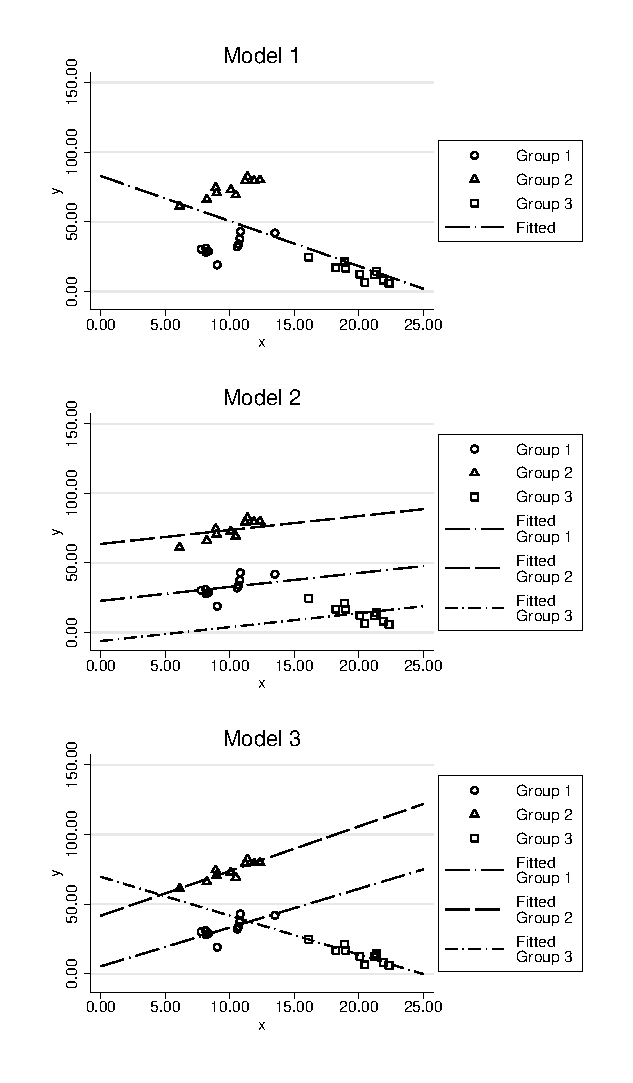
\includegraphics[angle=0,
           width=.75\textwidth]{interfit.eps}
   \caption{Scatter and fit plots of Models from data in Table~\ref{tab:groupxy}}
  \label{fig:interfit}
\end{figure}

\subsection{Example of a continuous-categorical interaction on math scores}

We return to the ECLS-K data on math scores for kindergartners. In these models we predict math scores based on two variables. The first variable is a dichotomous variable for school sector, $private$, coded 0 for public and 1 for private school. The next variable is $pared$, which is a standardized ($z$) score of parental education with a mean 0 and standard deviation of 1.

Model 1 in Table~\ref{tab:intereclscon} models math as a function of school sector
\[
y_i = \beta_0+\beta_1private_i+e_i
\]
Model 2 models math as a function of parental education
\[
y_i = \beta_0+\beta_1pared_i+e_i
\]
Model 3 models math as a function of school sector and parental education
\[
y_i = \beta_0+\beta_1private_i+\beta_2pared_i+e_i
\]
and finally, Model 4 tests whether school sector moderates the relationship between parental education and math scores
\[
y_i = \beta_0+\beta_1private_i+\beta_2pared_i+\beta_3\left(private_i \times pared_i\right)+e_i.
\]
\begin{table}[htbp]\centering
\caption{Models predicting math scores as a function of school sector and parental education
\label{tab:intereclscon}}
\begin{tabular}{lcccc}
\hline
Coefficients&Model 1&Model 2&Model 3&Model 4 \\
\hline
private   &    0.348***&        &    0.174***&    0.209***\\
      &   (0.023)  &        &   (0.023)  &   (0.024)  \\
pared    &        &    0.349***&    0.328***&    0.349***\\
      &        &   (0.011)  &   (0.011)  &   (0.012)  \\
private $\times$ pared&        &        &        &   -0.113***\\
      &        &        &        &   (0.028)  \\
Intercept    &   -0.077***&    0.000  &   -0.039***&   -0.036***\\
      &   (0.011)  &   (0.009)  &   (0.010)  &   (0.010)  \\

\hline
\multicolumn{5}{l}{Model Statistics} \\
\hline
$F$  &   228.079  &  1100.807  &   582.391  &   394.440  \\
$R^2$  &    0.021  &    0.093  &    0.098  &    0.100  \\
$df$ Regression 			 &    1.000  &    1.000  &    2.000  &    3.000  \\
$df$ Error 					 &  10694.000  &  10694.000  &  10693.000  &  10692.000  \\
\hline
\multicolumn{5}{l}{Math score and $pared$ standardized, N= 10696} \\
\multicolumn{5}{l}{$SE$s in parentheses, $***p<0.001$}
{\footnotesize{\emph{Source: ECLS-K}}} \\
\hline
\end{tabular}
\end{table}
We see in Model 1 that students who attend private schools have, on average, 0.348 standard deviations higher math scores than students who attend public schools. In Model 2, the data report that for each standard deviation increase in parental education, that math scores also increase about 0.349 standard deviations.

However, these effects are somewhat spurious, since when we combine the effects in Model 3, we find the effect of school sector reduced to almost half, while the effect of parental education remains. Model 4 offers some interesting information, however.

If we look at the model, we can calculate the "public" school relationship between parental education and math
\[
\hat{y} = \beta_0+\beta_1private+\beta_2pared+\beta_3\left(private \times pared\right)
\]
\[
\hat{y} = \beta_0+\beta_10+\beta_2pared+\beta_3\left(0 \times pared\right)
\]
\[
\hat{y} = \beta_0+\beta_2pared
\]
\[
\hat{y} = -0.036+0.349pared
\]
which shows that in {\it public} schools, parental education is a powerful predictor. In private schools, the effect of parental education is
\[
\hat{y} = \beta_0+\beta_11+\beta_2pared+\beta_3\left(1 \times pared\right)
\]
\[
\hat{y} = \left(\beta_0+\beta_1\right)+\left(\beta_2+\beta_3\right)pared
\]
\[
\hat{y} = \left(-0.036+0.209\right)+\left(0.349+-0.113\right)pared
\]
\[
\hat{y} = 0.173+0.236pared
\]
which means that in {\it private} schools, the effect of parental education is less, 0.236, than in {\it public} schools, 0.349. However, the intercept is also larger in private schools.

\section{Interactions between continuous predictors}

Interactions between continuous predictors are often tricky to understand. My strategy is to fit the model with continuous predictors, but then convert one variable into a quasi-categorical variable during interpretation. My method to make this easier is to convert one of the variables in used in the interaction into a $z$ score; usually the proposed moderating variable.

The model for a continuous interaction is like any other model with interactions. The outcome $y$ is predicted with (along with controls) two variables $x$ and $z$, and the product of $x$ and $z$, $x\times z$
\[
y_i=\beta_0+\beta_1x_i+\beta_2z_i+\beta_3\left(x_i\times z_i\right)+e_i
\]
The trick to visualizing how the moderation affects the regression lines is to pick three values for $z$, and if $z$ is standardized, natural candidates are (a) one standard deviation below the mean, -1, (b) the mean, 0, and (c) one standard deviation above the mean, 1. Thus, the regression line for one standard deviation below the mean is
\[
\hat{y}=\beta_0+\beta_1+\beta_2\left(-1\right)+\beta_3\left(x\times -1\right)
\]
\[
\hat{y}=\beta_0+\beta_1x-\beta_2-\beta_3x
\]
\[
\hat{y}=\left(\beta_0-\beta_2\right)+\left(\beta_1-\beta_3\right)x
\]
the regression line for the mean is
\[
\hat{y}=\beta_0+\beta_1+\beta_2\left(0\right)+\beta_3\left(x\times 0\right)
\]
\[
\hat{y}=\beta_0+\beta_1x
\]
and the regression line for one standard deviation above the mean is
\[
\hat{y}=\beta_0+\beta_1+\beta_2\left(1\right)+\beta_3\left(x\times 1\right)
\]
\[
\hat{y}=\beta_0+\beta_1x+\beta_2+\beta_3x
\]
\[
\hat{y}=\left(\beta_0+\beta_2\right)+\left(\beta_1+\beta_3\right)x.
\]

\subsection{Example of a continuous-continuous interaction on income}

In this example we will use data from the 2008 GSS to estimate how income is affected by the prestige of someone's job verses their level of education. Our running hypothesis is that the prestige moderates the impact of education on income.

Income in the GSS is measured categorically, with $\geq$ 25 thousand dollars as the top category. Just as we did in \ref{sec:midpointref} (see footnote), I mid-pointed the categories to create a continuous variable. Table~\ref{tab:incomeprestige} presents four models. The first model predicts income as a function of the standardized prestige, $z$
\[
y_i=\beta_0+\beta_1prestige_i+e_i
\]
Model 2 predicts income as a function of years of education
\[
y_i=\beta_0+\beta_1educ_i+e_i
\]
Model 3 predicts income as a function of both prestige and years of education
\[
y_i=\beta_0+\beta_1prestige_i+\beta_2educ_i+e_i
\]
and finally, Model 4 includes the interaction of prestige and years of education
\[
y_i=\beta_0+\beta_1prestige_i+\beta_2educ_i+\beta_3\left(prestige_i\times educ_i\right)+e_i.
\]
\begin{table}[htbp]\centering
\caption{Models predicting income in thousands as a function of occupational prestige and education
\label{tab:incomeprestige}}
\begin{tabular}{lcccc}
\hline
Coefficients&Model 1&Model 2&Model 3&Model 4 \\
\hline
prestige  &    1.529***&        &    0.813***&    4.767***\\
      &   (0.120)  &        &   (0.138)  &   (0.594)  \\
educ    &        &    0.629***&    0.460***&    0.448***\\
      &        &   (0.041)  &   (0.048)  &   (0.047)  \\
prestige $\times$ educ &        &        &        &   -0.273***\\
      &        &        &        &   (0.040)  \\
Intercept    &   22.250***&   13.515***&   15.940***&   16.532***\\
      &   (0.120)  &   (0.570)  &   (0.663)  &   (0.662)  \\
\hline
\multicolumn{5}{l}{Model Statistics} \\
\hline
$F$   &   163.625  &   238.865  &   131.906  &   105.361  \\
$R^2$  &    0.068  &    0.093  &    0.106  &    0.124  \\
$df$ Regression 			 &    1.000  &    1.000  &    2.000  &    3.000  \\
$df$ Error 					  &  2234.000  &  2332.000  &  2232.000  &  2231.000  \\
\hline
\multicolumn{5}{l}{prestige standardized, $N= 2236$} \\
\multicolumn{5}{l}{$SE$s in parentheses, $***p<0.001$}
{\footnotesize{\emph{Source: GSS 2008}}} \\
\hline
\end{tabular}
\end{table}
\begin{figure}
   \centering
   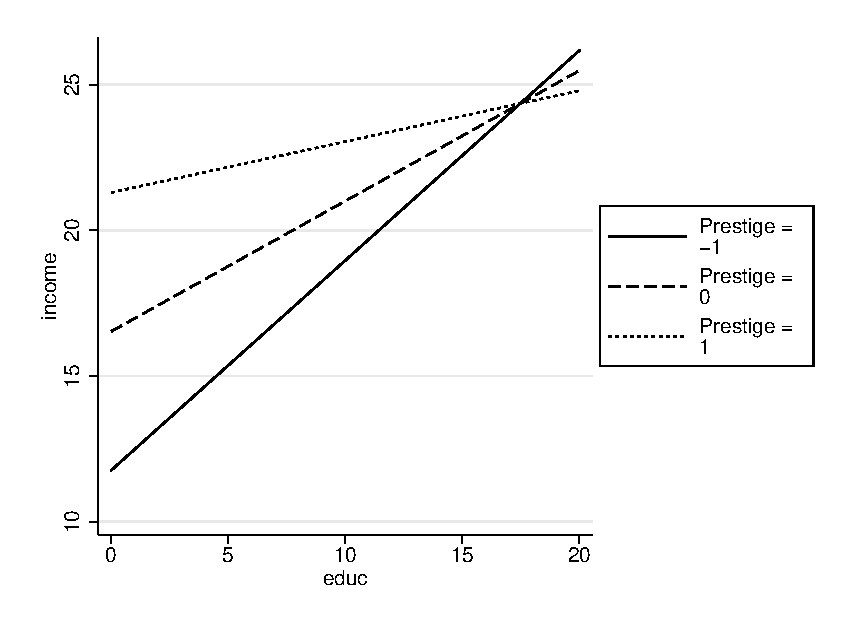
\includegraphics[angle=0,
           width=.75\textwidth]{gssedupres.eps}
   \caption{Income as a function of education by prestige of occupation from Model 4 in Table~\ref{tab:incomeprestige}}
  \label{fig:gssedupres}
\end{figure}

Looking at Model 1, and noting the prestige is a standardized variable and that income is measured in thousands, we see that for each standard deviation increase in prestige, annual income increases by about 1,529 dollars, with an average income of about 22,250 dollars. An examination of Model 2 indicates that for each year of education, annual income increases by about 629 dollars.

Model 3 estimates the effect of education, holding constant the effects of occupational prestige. We see the effect of prestige is smaller when we control for education, this time showing only a 813 dollar increase for each standard deviation increase in prestige. The effect is also reduced, showing only a 460 dollar increase for each year of education.

We now turn to Model 4, which includes the interaction of $\left(prestige \times educ\right)$, we can focus on the effect of education for different levels of prestige. Since prestige is standardized, we can pick three levels of prestige: (a) one standard deviation below the mean, -1, (b) the mean, 0, and (c) one standard deviation above the mean, 1.

First, we figure out the model for education where prestige = -1
\[
\hat{y}=\beta_0+\beta_1prestige+\beta_2educ+\beta_3\left(prestige\times educ\right)
\]
\[
\hat{y}=\beta_0+\beta_1-1+\beta_2educ+\beta_3\left(-1\times educ\right)
\]
\[
\hat{y}=\beta_0-\beta_1+\beta_2educ-\beta_3educ
\]
\[
\hat{y}=\left(\beta_0-\beta_1\right)+\left(\beta_2-\beta_3\right)educ
\]
\[
\hat{y}=\left(16.532-4.767\right)+\left(0.448--0.273\right)educ
\]
\[
\hat{y}=11.765+0.721educ
\]
Next, the model for education where prestige = 0 (the mean)
\[
\hat{y}=\beta_0+\beta_1prestige+\beta_2educ+\beta_3\left(prestige\times educ\right)
\]
\[
\hat{y}=\beta_0+\beta_10+\beta_2educ+\beta_3\left(0\times educ\right)
\]
\[
\hat{y}=\beta_0+\beta_2educ
\]
\[
\hat{y}=16.532+0.448educ
\]
Finally, the model for education where prestige = 1
\[
\hat{y}=\beta_0+\beta_1prestige+\beta_2educ+\beta_3\left(prestige\times educ\right)
\]
\[
\hat{y}=\beta_0+\beta_11+\beta_2educ+\beta_3\left(1\times educ\right)
\]
\[
\hat{y}=\beta_0+\beta_1+\beta_2educ+\beta_3educ
\]
\[
\hat{y}=\left(\beta_0+\beta_1\right)+\left(\beta_2+\beta_3\right)educ
\]
\[
\hat{y}=\left(16.532+4.767\right)+\left(0.448+-0.273\right)educ
\]
\[
\hat{y}=21.299+0.175educ
\]
Note that, substantively, when occupational prestige is low (-1), the intercept is also low, but the effect of education is strong. When prestige is average (0), the intercept is higher, signaling that pay is somewhat better, but the returns on education are lower (lower slope). Finally, when prestige is high (1), the intercept is even higher and the effects of education are lower still. Of course, this all makes sense. These patterns are visualized in Figure~\ref{fig:gssedupres}. 